\documentclass{beamer}
\setbeamertemplate{caption}[numbered]
\usepackage{tikz}
\usepackage{pgfplots}
\usepackage{color}
\usepackage{listings}
\lstset{basicstyle=\ttfamily,
showstringspaces=false,
commentstyle=\color{red},
keywordstyle=\color{blue}}
\usetheme{Goettingen}
\title{Introduction to Deep Learning and Caffe}
\author{HE Shuncheng\\hsc12@outlook.com}
\institute{Tsinghua-Seagate Future Robotics Club \\ Association of Science and Technology of Automation}
\date{\today}
\begin{document}

\begin{frame}
	\titlepage   
\end{frame}

\begin{frame}
	\frametitle{Contents}
	\tableofcontents
\end{frame}

\section{Classification Task}
\begin{frame}
	\frametitle{Binary Classification}	
\begin{minipage}[h]{.5\textwidth}
\begin{figure}[htbp]
\centerline{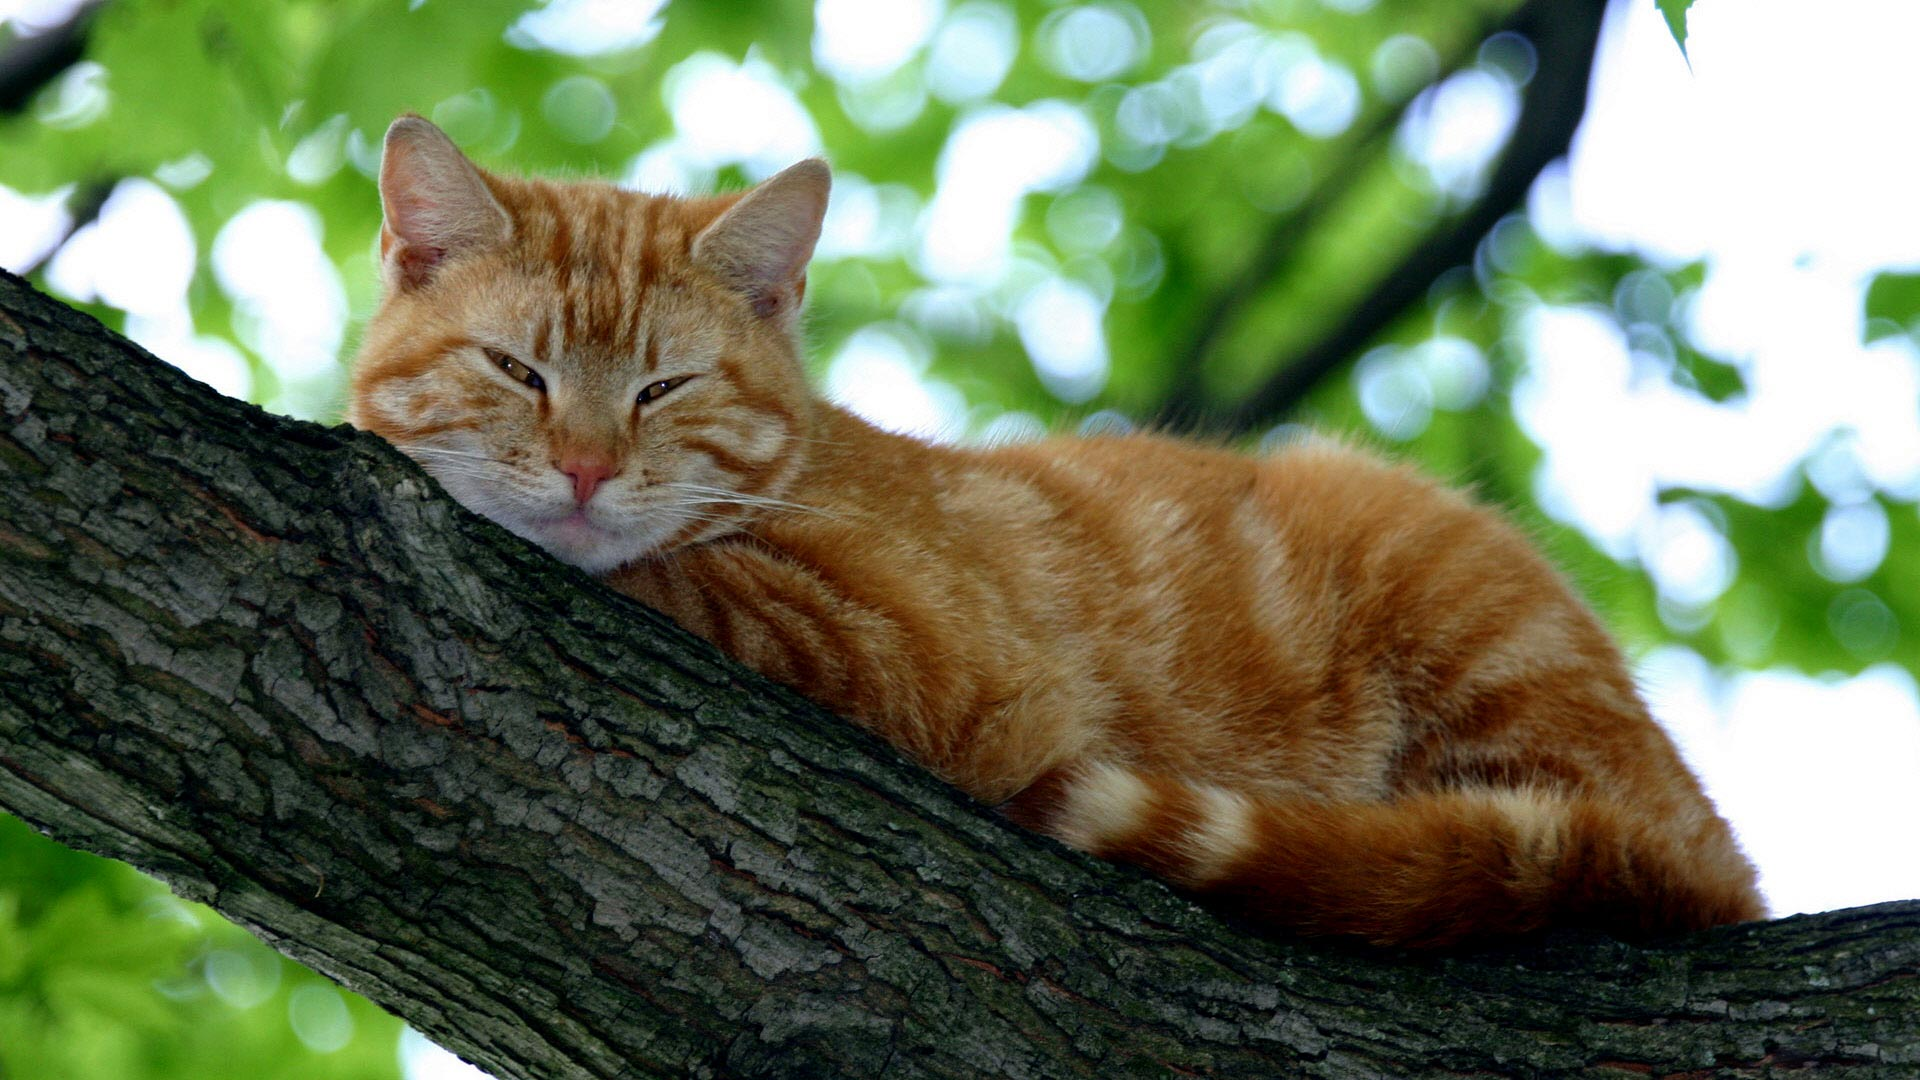
\includegraphics[width=1in]{cat.jpg}}
\caption[1]{a cat?}
\end{figure}
\end{minipage}%
\begin{minipage}[h]{.5\textwidth}
\begin{figure}[htbp]
\centerline{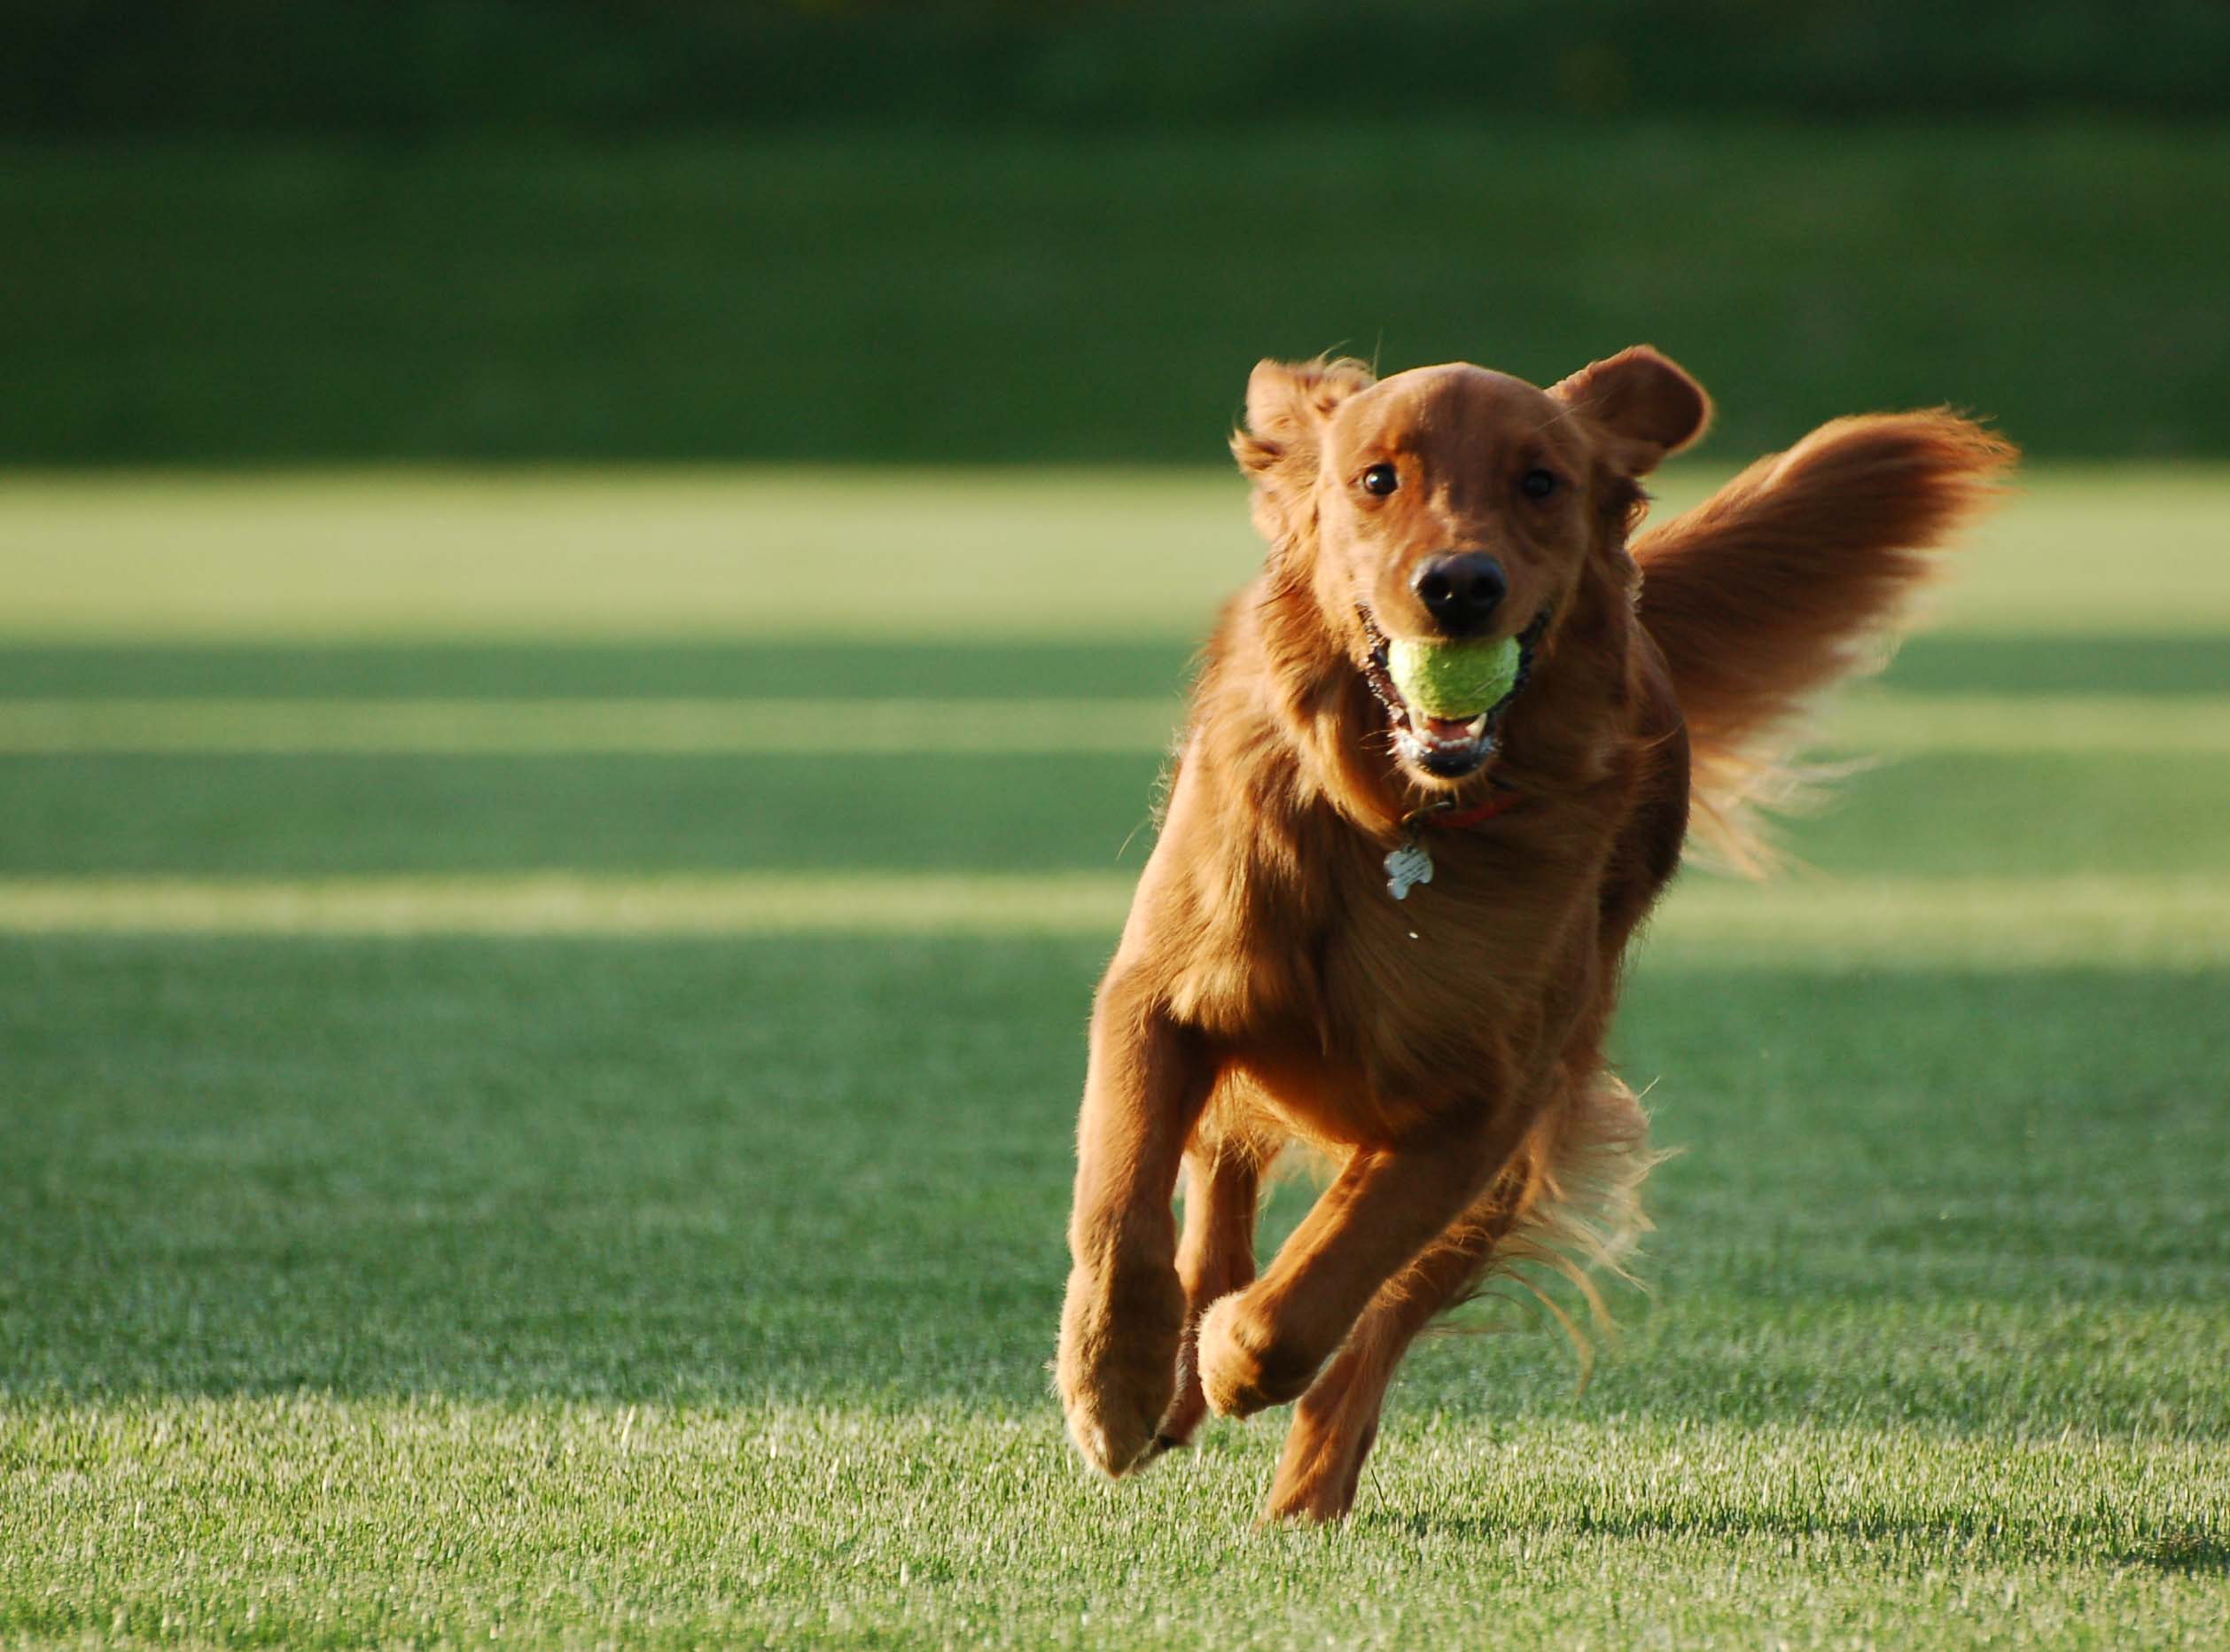
\includegraphics[width=1in]{dog.jpg}}
\caption[2]{a dog?}
\end{figure}
\end{minipage}
\textbf{Binary Classification}: Given input data $x$ (e.g. a picture), the output of a binary classifier $y=f(x)$ is one label retrieved from a set of two labels $y\in\{\pm1\}$.
\end{frame}

\begin{frame}
\frametitle{Linear Classifier}
\begin{minipage}[h]{.5\textwidth}
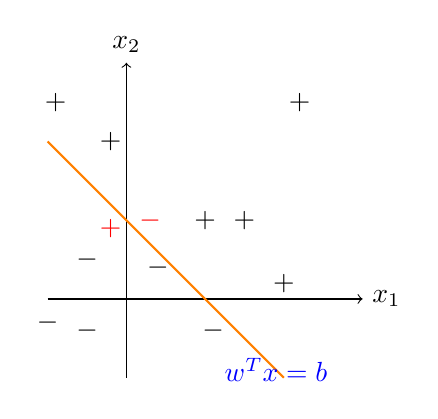
\begin{tikzpicture}
\draw[->] (-1,0) -- (3,0);
\draw[->] (0,-1) -- (0,3);
\draw[orange, thick] (-1,2) -- (2,-1);
\node[right] at (3,0) {$x_{1}$};
\node[above] at (0,3) {$x_{2}$};
\node[] at (1,1) {$+$};
\node[] at (1.5,1) {$+$};
\node[] at (2,0.2) {$+$};
\node[] at (-1,-0.3) {$-$};
\node[] at (-0.5,-0.4) {$-$};
\node[] at (0.4,0.4) {$-$};
\node[] at (-0.2,2) {$+$};
\node[] at (2.2,2.5) {$+$};
\node[] at (1.1,-0.4) {$-$};
\node[] at (-0.9,2.5) {$+$};
\node[] at (-0.5,0.5) {$-$};
\node[blue] at (1.9,-0.9) {$w^{T}x=b$};
\node[red] at (0.3,1) {$-$};
\node[red] at (-0.2,0.9) {$+$};
\end{tikzpicture}
\end{minipage}%
\begin{minipage}[h]{.5\textwidth}
Data set $\mathcal{D}=$\\
$\{(x_{1}^{(1)},x_{2}^{(1)}),\cdots,(x_{1}^{(n)},x_{2}^{(n)})\}$\\
A linear binary classifier is a\\
hyperplane $w^{T}x=b$\\
$f(x)=sgn(w^{T}x-b)$
\end{minipage}
\end{frame}

\begin{frame}
\frametitle{Performance of Linear Classifier}
\begin{minipage}[h]{.6\textwidth}
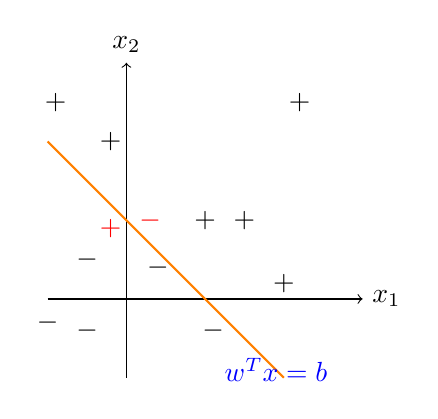
\begin{tikzpicture}
\draw[->] (-1,0) -- (3,0);
\draw[->] (0,-1) -- (0,3);
\draw[orange, thick] (-1,2) -- (2,-1);
\node[right] at (3,0) {$x_{1}$};
\node[above] at (0,3) {$x_{2}$};
\node[] at (1,1) {$+$};
\node[] at (1.5,1) {$+$};
\node[] at (2,0.2) {$+$};
\node[] at (-1,-0.3) {$-$};
\node[] at (-0.5,-0.4) {$-$};
\node[] at (0.4,0.4) {$-$};
\node[] at (-0.2,2) {$+$};
\node[] at (2.2,2.5) {$+$};
\node[] at (1.1,-0.4) {$-$};
\node[] at (-0.9,2.5) {$+$};
\node[] at (-0.5,0.5) {$-$};
\node[blue] at (1.9,-0.9) {$w^{T}x=b$};
\node[red] at (0.3,1) {$-$};
\node[red] at (-0.2,0.9) {$+$};
\end{tikzpicture}
\end{minipage}%
\begin{minipage}[h]{.4\textwidth}
\textbf{True Positive}: \\
$y=+1, f(x)=+1$\\
\textbf{True Negative}: \\
$y=-1, f(x)=-1$\\
\textbf{False Positive}: \\
$y=-1, f(x)=+1$\\
\textbf{False Negative}: \\
$y=+1, f(x)=-1$\\
\textbf{Accuracy}: \\
$\frac{TP+TN}{n}$\\
\textbf{Error Rate}: \\
$\frac{FP+FN}{n}$
\end{minipage}
\phantom{anything}\\
\vspace{10pt}
A good classifier: \textbf{minizing} the error rate
\end{frame}

\begin{frame}
\frametitle{Basic Concepts}
\begin{minipage}[h]{.6\textwidth}
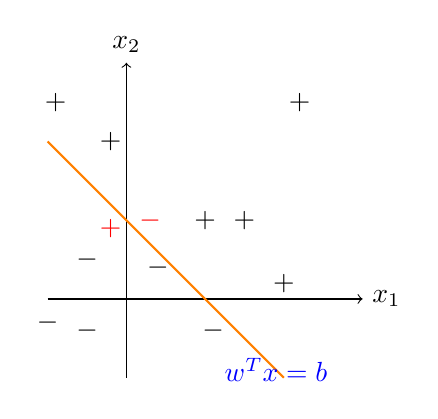
\begin{tikzpicture}
\draw[->] (-1,0) -- (3,0);
\draw[->] (0,-1) -- (0,3);
\draw[orange, thick] (-1,2) -- (2,-1);
\node[right] at (3,0) {$x_{1}$};
\node[above] at (0,3) {$x_{2}$};
\node[] at (1,1) {$+$};
\node[] at (1.5,1) {$+$};
\node[] at (2,0.2) {$+$};
\node[] at (-1,-0.3) {$-$};
\node[] at (-0.5,-0.4) {$-$};
\node[] at (0.4,0.4) {$-$};
\node[] at (-0.2,2) {$+$};
\node[] at (2.2,2.5) {$+$};
\node[] at (1.1,-0.4) {$-$};
\node[] at (-0.9,2.5) {$+$};
\node[] at (-0.5,0.5) {$-$};
\node[blue] at (1.9,-0.9) {$w^{T}x=b$};
\node[red] at (0.3,1) {$-$};
\node[red] at (-0.2,0.9) {$+$};
\end{tikzpicture}
\end{minipage}%
\begin{minipage}[h]{.4\textwidth}
\textbf{Training Set}\\
\textbf{Test Set}\\
\textbf{Training Error}\\
\textbf{Generalization Error}\\
\textbf{Overfitting}\\
\textbf{Loss Function}
\end{minipage}
\phantom{anything}\\
\vspace{10pt}
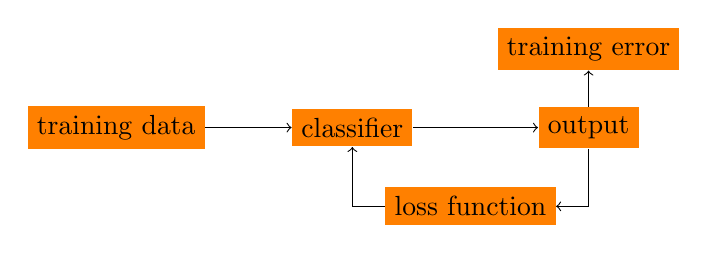
\begin{tikzpicture}
\node[fill=orange] (a) at (0,0) {training data};
\node[fill=orange] (b) at (3,0) {classifier};
\draw[->] (a) -- (b);
\node[fill=orange] (c) at (6,0) {output};
\draw[->] (b) -- (c);
\node[fill=orange] (d) at (4.5,-1) {loss function};
\draw[->] (c) |- (d);
\draw[->] (d) -| (b);
\node[fill=orange] (e) at (6,1) {training error};
\draw[->] (c) -- (e);
\end{tikzpicture}
\end{frame}

\begin{frame}
\frametitle{Overfitting}
\begin{minipage}[h]{.45\textwidth}
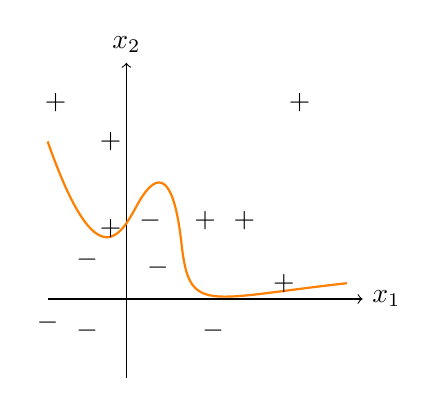
\begin{tikzpicture}
\draw[->] (-1,0) -- (3,0);
\draw[->] (0,-1) -- (0,3);
\draw[orange, thick] (-1,2) .. controls (-0.3,0) and (0,1) .. (0.2,1.3);
\draw[orange, thick] (0.2,1.3) .. controls (0.4,1.6) and (0.6,1.6) .. (0.7,0.7);
\draw[orange, thick] (0.7,0.7) .. controls (0.8,-0.2) and (1,0) .. (2.8,0.2);
\node[right] at (3,0) {$x_{1}$};
\node[above] at (0,3) {$x_{2}$};
\node[] at (1,1) {$+$};
\node[] at (1.5,1) {$+$};
\node[] at (2,0.2) {$+$};
\node[] at (-1,-0.3) {$-$};
\node[] at (-0.5,-0.4) {$-$};
\node[] at (0.4,0.4) {$-$};
\node[] at (-0.2,2) {$+$};
\node[] at (2.2,2.5) {$+$};
\node[] at (1.1,-0.4) {$-$};
\node[] at (-0.9,2.5) {$+$};
\node[] at (-0.5,0.5) {$-$};
\node[] at (0.3,1) {$-$};
\node[] at (-0.2,0.9) {$+$};
\end{tikzpicture}
\end{minipage}%
\begin{minipage}[h]{.55\textwidth}
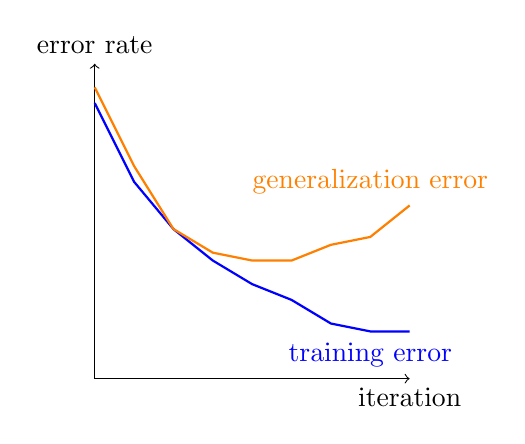
\begin{tikzpicture}
\draw[->] (0,0) -- (4,0);
\draw[->] (0,0) -- (0,4);
\node[below] at (4,0) {iteration};
\node[above] at (0,4) {error rate};
\draw[blue, thick] (0,3.5) -- (0.5,2.5) -- (1,1.9) -- (1.5,1.5) -- (2,1.2) -- (2.5,1) -- (3,0.7) -- (3.5,0.6) -- (4,0.6);
\draw[orange, thick] (0,3.7) -- (0.5,2.7) -- (1,1.9) -- (1.5,1.6) -- (2,1.5) -- (2.5,1.5) -- (3,1.7) -- (3.5,1.8) -- (4,2.2);
\node[blue] at (3.5,0.3) {training error};
\node[orange] at (3.5,2.5) {generalization error};
\end{tikzpicture}
\end{minipage}
\end{frame}

\section{Structure of ANN}
\begin{frame}
\frametitle{Perceptron}
\begin{tikzpicture}
\draw (0,3) -- (3,1.5);
\draw (0,2) -- (3,1.5);
\draw (0,0) -- (3,1.5);
\draw (2,3.5) -- (3,1.5);
\draw[->] (3,1.5) -- (8.7,1.5);
\node[above] at (2,3.5) {$x_{0}=1$};
\fill[orange] (0,3) circle (0.3);
\fill[orange] (0,2) circle (0.3);
\fill[orange] (0,0) circle (0.3);
\fill (0,1.15) circle (0.04);
\fill (0,1) circle (0.04);
\fill (0,0.85) circle (0.04);
\fill[white] (3,1.5) circle (0.5);
\draw[orange, thick] (3,1.5) circle (0.5);
\node[] at (3,1.5) {$\sum$};
\node[] at (0,3) {$x_{1}$};
\node[] at (0,2) {$x_{2}$};
\node[] at (0,0) {$x_{n}$};
\node[] at (1,2.7) {$w_{1}$};
\node[] at (1,2) {$w_{2}$};
\node[] at (1,0.7) {$w_{n}$};
\node[] at (2.7,2.7) {$w_{0}$};
\fill[white] (6,1.5) circle (0.5);
\draw[orange, thick] (6,1.5) circle (0.5);
\draw (5.6,1.5) -- (6.4,1.5);
\draw (6,1.1) -- (6,1.9);
\draw[orange, thick] (5.6,1.2) -- (6,1.2) -- (6,1.8) -- (6.4,1.8);
\node[below] at (4.5,1.5) {$\sum_{i=0}^{n}w_{i}x_{i}$};
\fill[orange] (9,1.5) circle (0.3);
\node[] at (9,1.5) {$y$};
\node[] at (7,0) {%
$y=\left\{
\begin{aligned}
+1&,if\hspace{6pt}w^{T}x>0 \\
-1&,otherwise
\end{aligned}
\right.$};
\end{tikzpicture}
\end{frame}

\begin{frame}
\frametitle{Perceptron}
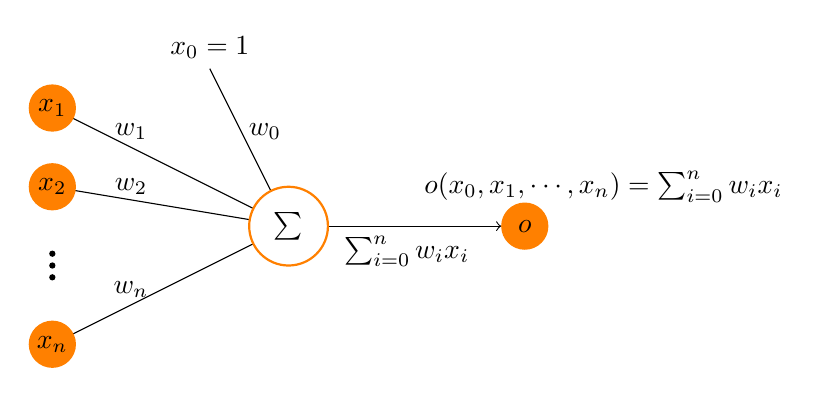
\begin{tikzpicture}
\draw (0,3) -- (3,1.5);
\draw (0,2) -- (3,1.5);
\draw (0,0) -- (3,1.5);
\draw (2,3.5) -- (3,1.5);
\draw[->] (3,1.5) -- (5.7,1.5);
\node[above] at (2,3.5) {$x_{0}=1$};
\fill[orange] (0,3) circle (0.3);
\fill[orange] (0,2) circle (0.3);
\fill[orange] (0,0) circle (0.3);
\fill (0,1.15) circle (0.04);
\fill (0,1) circle (0.04);
\fill (0,0.85) circle (0.04);
\fill[white] (3,1.5) circle (0.5);
\draw[orange, thick] (3,1.5) circle (0.5);
\node[] at (3,1.5) {$\sum$};
\node[] at (0,3) {$x_{1}$};
\node[] at (0,2) {$x_{2}$};
\node[] at (0,0) {$x_{n}$};
\node[] at (1,2.7) {$w_{1}$};
\node[] at (1,2) {$w_{2}$};
\node[] at (1,0.7) {$w_{n}$};
\node[] at (2.7,2.7) {$w_{0}$};
\node[below] at (4.5,1.5) {$\sum_{i=0}^{n}w_{i}x_{i}$};
\fill[orange] (6,1.5) circle (0.3);
\node[] at (6,1.5) {$o$};
\node[] at (7,2) {%
$o(x_{0},x_{1},\cdots,x_{n})=\sum_{i=0}^{n}w_{i}x_{i}$};
\end{tikzpicture}
\end{frame}

\begin{frame}
\frametitle{Training Algorithm}
Define a loss function:\\
\begin{equation*}
E(w)=\frac{1}{2}\sum_{d\in\mathcal{D}}(t_{d}-o_{d})^{2}
\end{equation*}\\
How to reduce loss?\\
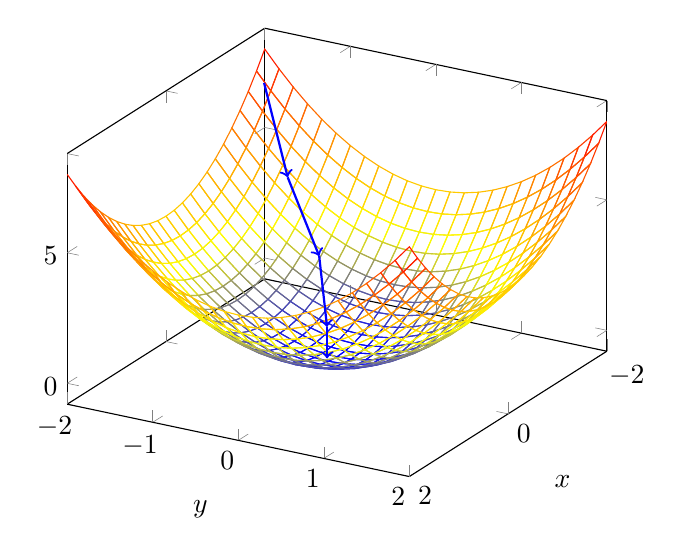
\begin{tikzpicture}
\begin{axis}[view={120}{30},xlabel=$x$,ylabel=$y$]
\addplot3[domain=-2:2,y domain=-2:2,mesh]{x^2+y^2};
\end{axis}
\draw[blue, thick, ->] (2.5,5) -- (2.8,3.8);
\draw[blue, thick, ->] (2.8,3.8) -- (3.2,2.8);
\draw[blue, thick, ->] (3.2,2.8) -- (3.3,1.9);
\draw[blue, thick, ->] (3.3,1.9) -- (3.3,1.5);
\end{tikzpicture}
\end{frame}

\begin{frame}
\frametitle{Gradient Descent}
Gradient w.r.t. $w$\\
\begin{equation*}
\nabla E(w)=(\frac{\partial E}{\partial w_{0}},\frac{\partial E}{\partial w_{1}},\cdots,\frac{\partial E}{\partial w_{n}})^{T}
\end{equation*}\\
where\\
\begin{equation*}
\frac{\partial E}{\partial w_{i}}=\sum_{d\in\mathcal{D}}(t_{d}-o_{d})(-x_{i}^{(d)})
\end{equation*}
for every iteration ($\eta$ denotes learning rate)\\
\begin{equation*}
w_{i}\gets w_{i}+\Delta w_{i}
\end{equation*}
\begin{equation*}
\Delta w_{i}=-\eta\frac{\partial E}{\partial w_{i}}=\eta\sum_{d\in\mathcal{D}}(t_{d}-o_{d})x_{i}^{(d)}
\end{equation*}
\begin{equation*}
\forall i\in[n]
\end{equation*}
\end{frame}

\begin{frame}
\frametitle{Artificial Neural Network}
Structure of ANN\\
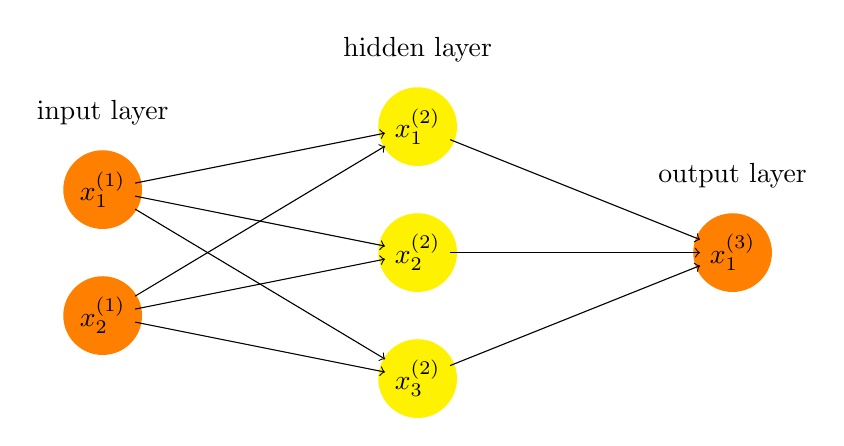
\begin{tikzpicture}
\fill[orange] (0,0.8) circle (0.5); 
\fill[orange] (0,-0.8) circle (0.5);
\fill[yellow] (4,1.6) circle (0.5);
\fill[yellow] (4,0) circle (0.5);
\fill[yellow] (4,-1.6) circle (0.5);
\fill[orange] (8,0) circle (0.5);
\node[] (x11) at (0,0.8) {$x_{1}^{(1)}$};
\node[] (x21) at (0,-0.8) {$x_{2}^{(1)}$};
\node[] (x12) at (4,1.6) {$x_{1}^{(2)}$};
\node[] (x22) at (4,0) {$x_{2}^{(2)}$};
\node[] (x32) at (4,-1.6) {$x_{3}^{(2)}$};
\node[] (x13) at (8,0) {$x_{1}^{(3)}$};
\draw[->] (x11) -- (x12);
\draw[->] (x12) -- (x13);
\draw[->] (x11) -- (x22);
\draw[->] (x22) -- (x13);
\draw[->] (x11) -- (x32);
\draw[->] (x32) -- (x13);
\draw[->] (x21) -- (x12);
\draw[->] (x21) -- (x22);
\draw[->] (x21) -- (x32);
\node[above=20pt] at (x11) {input layer};
\node[above=20pt] at (x12) {hidden layer};
\node[above=20pt] at (x13) {output layer};
\end{tikzpicture}
\begin{equation*}
x^{l+1}=h((W^{l})^{T}x^{l})
\end{equation*}
$h$ is a non-linear function.
\end{frame}

\begin{frame}
\frametitle{Sigmoid Function}
\begin{equation*}
h(x)=\frac{1}{1+e^{-x}}
\end{equation*}\\
\begin{tikzpicture}
\draw[->] (-4,0) -- (4,0) node[below] {$x$};
\draw[->] (0,-0.5) -- (0,2.5) node[above] {$h(x)$};
\draw[orange,thick,domain=-4:4] plot(\x,{2/(1+e^(-\x))});
\draw[dashed] (-4,2) -- (4,2);
\node[anchor=south east,inner sep=0] at (0,2) {1};
\node[anchor=north east,inner sep=0] at (0,0) {0};
\end{tikzpicture}
\begin{itemize}
\item 1. continuous, differentiable
\item 2. map $[-\infty,+\infty]$ to $[0,1]$
\item 3. nonlinearity
\item 4. $h'(x)$ is easy to calculate
\end{itemize}
\begin{equation*}
h'(x)=h(x)(1-h(x))
\end{equation*}
\end{frame}

\begin{frame}
\frametitle{Back Propagation and Delta Rule}
Please refer to \href{http://caffe.stevenho.me/cnn_tutorial.pdf}{\color{blue}{this page}}\par
Mathematical model of ANN
\begin{equation*}
x^{l}=f(u^{l}), u^{l}=(W^{l-1})^{T}x^{l-1}
\end{equation*}
where $l$ denotes the current layer with the output layer designated to be layer $L$ and the input layer desiganted to ba layer $1$. Function $f(\cdot)$ is a nonlinear function (i.e. sigmoid or hyperbolic tangent).\par
Define loss function as
\begin{equation*}
E(x^{L},t)
\end{equation*}
where $x^{L}$ is the network output and $t$ is the target output.
\end{frame}

\begin{frame}
\frametitle{Back Propagation and Delta Rule}
Expand the loss function
\begin{equation*}
E(x^{L},t)=E(f((W^{L-1})^{T}x^{L-1}),t)
\end{equation*}
Using chain rule, we can write the derivatives w.r.t. $W^{L-1}$\par
\begin{equation*}
\frac{\partial E}{\partial W^{L-1}}=x^{L-1}(f'(u^{L})\star\frac{\partial E}{\partial x^{L}})^{T}
\end{equation*}\par
where $\star$ denotes elementwise multiplication, and if we define\par
\begin{equation*}
\delta^{L}=f'(u^{L})\star\frac{\partial E}{\partial x^{L}}
\end{equation*}\par
we get\par
\begin{equation*}
\frac{\partial E}{\partial W^{L-1}}=x^{L-1}(\delta^{L})^{T}
\end{equation*}\par
\end{frame}

\begin{frame}
\frametitle{Back Propagation and Delta Rule}
If we calculate the $\delta$ term recursively
\begin{equation*}
\delta^{l}=f'(u^{l})\star((W^{l})^{T}\delta^{l+1}),l=L-1,\cdots,2
\end{equation*}
it is easy to write
\begin{equation*}
\frac{\partial E}{\partial W^{l}}=x^{l}(\delta^{l+1})^{T},l=L-2,\cdots,1
\end{equation*}
\end{frame}

\section{CNN for Image Classification}
\begin{frame}[label=struct1]
\frametitle{Network Structure}
\begin{figure}[htbp]
\centerline{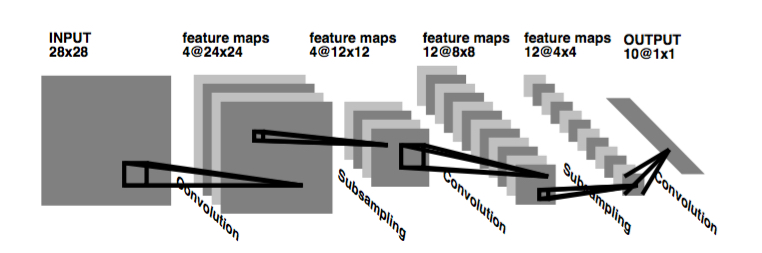
\includegraphics[width=\textwidth]{lenet.jpg}}
\caption[3]{structure of convolutional neural network}
\end{figure}\par
\begin{itemize}
\item \hyperlink{conv1}{Convolution Layer}
\item \hyperlink{pool}{Pooling Layer (Subsampling)}
\item \hyperlink{ip}{Full-connected Layer (Inner-product)}
\item \hyperlink{relu}{ReLU Layer}
\item \hyperlink{softmax}{Softmax Layer}
\end{itemize}
\end{frame}

\begin{frame}[label=conv1]
\frametitle{Convolution Layer}
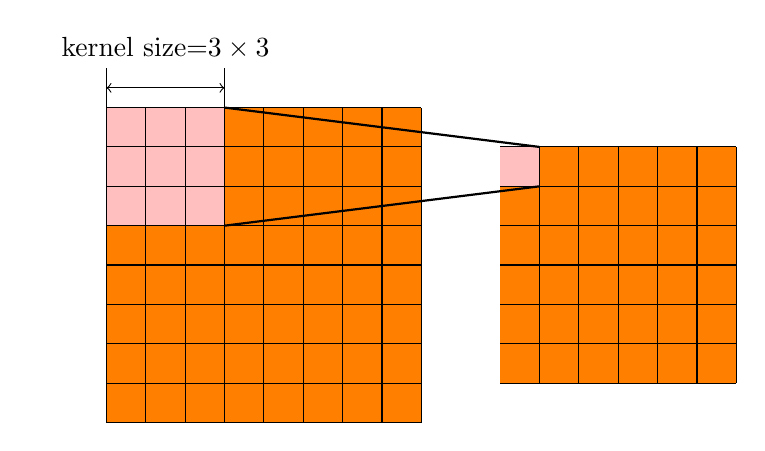
\begin{tikzpicture}
\fill[orange] (0,0) rectangle (4,4);
\fill[pink] (0,2.5) rectangle (1.5,4);
\fill[white] (-1,4.5) rectangle (0,5);
\draw[step=0.5] (0,0) grid (4,4);
\draw[<->] (0,4.25) -- (1.5,4.25);
\draw[] (0,4) -- (0,4.5);
\draw[] (1.5,4) -- (1.5,4.5);
\node[above] at (0.75,4.5) {kernel size=$3\times 3$};
\fill[orange] (5,0.5) rectangle (8,3.5);
\fill[pink] (5,3) rectangle (5.5,3.5);
\draw[step=0.5] (5,0.5) grid (8,3.5);
\draw[thick] (1.5,4) -- (5.5,3.5);
\draw[thick] (1.5,2.5) -- (5.5,3);
\end{tikzpicture}\par
\begin{equation*}
g_{ij}=\sum_{s=i}^{i+2}\sum_{t=j}^{j+2}h_{st}k_{st}
\end{equation*}
\end{frame}

\begin{frame}[label=conv2]
\frametitle{Convolution Layer}
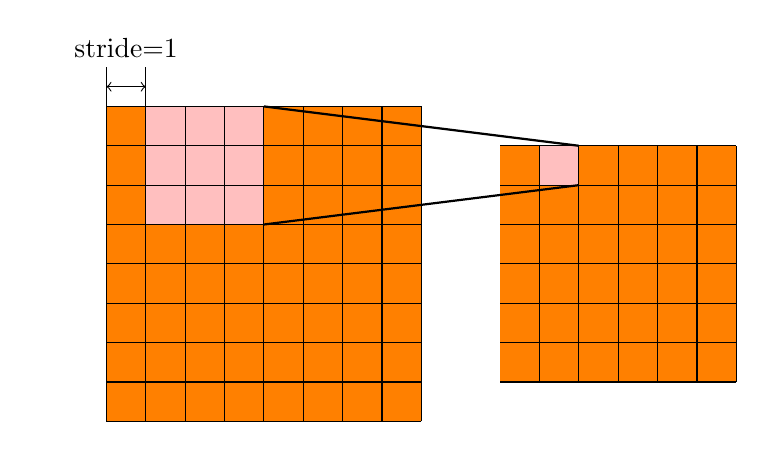
\begin{tikzpicture}
\fill[orange] (0,0) rectangle (4,4);
\fill[pink] (0.5,2.5) rectangle (2,4);
\fill[white] (-1,4.5) rectangle (0,5);
\draw[step=0.5] (0,0) grid (4,4);
\draw[<->] (0,4.25) -- (0.5,4.25);
\draw[] (0,4) -- (0,4.5);
\draw[] (0.5,4) -- (0.5,4.5);
\node[above] at (0.25,4.5) {stride=1};
\fill[orange] (5,0.5) rectangle (8,3.5);
\fill[pink] (5.5,3) rectangle (6,3.5);
\draw[step=0.5] (5,0.5) grid (8,3.5);
\draw[thick] (2,4) -- (6,3.5);
\draw[thick] (2,2.5) -- (6,3);
\end{tikzpicture}\par
\begin{equation*}
g_{ij}=\sum_{s=i}^{i+2}\sum_{t=j}^{j+2}h_{st}k_{st}
\end{equation*}
\end{frame}

\begin{frame}[label=pool]
\frametitle{Pooling Layer}
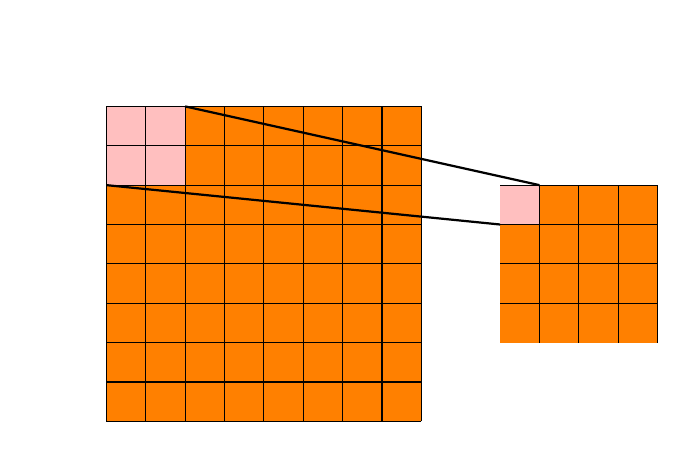
\begin{tikzpicture}
\fill[orange] (0,0) rectangle (4,4);
\fill[pink] (0,3) rectangle (1,4);
\fill[white] (-1,4.5) rectangle (0,5);
\draw[step=0.5] (0,0) grid (4,4);
\fill[orange] (5,1) rectangle (7,3);
\fill[pink] (5,2.5) rectangle (5.5,3);
\draw[step=0.5] (5,1) grid (7,3);
\draw[thick] (1,4) -- (5.5,3);
\draw[thick] (0,3) -- (5,2.5);
\end{tikzpicture}\par
\begin{equation*}
g_{ij}=\max\{h_{2i,2j},h_{2i+1,2j},h_{2i,2j+1},h_{2i+1,2j+1}\}
\end{equation*}\par
\textbf{No free parameter} in pooling layer. 
\end{frame}

\begin{frame}[label=ip]
\frametitle{Inner-product}
Known as full-connected layer. Weights are designated from every input to every output, namely
\begin{equation*}
y=W^{T}x
\end{equation*}
\end{frame}

\begin{frame}[label=relu]
\frametitle{Rectified Linear Unit}
\begin{minipage}[h]{.5\textwidth}
A rectifier
\begin{equation*}
y=\max\{0,x\}
\end{equation*}
A rectified linear unit
\begin{equation*}
y=ln(1+e^{x})
\end{equation*}
with its derivative w.r.t. $x$
\begin{equation*}
\frac{dy}{dx}=\frac{1}{1+e^{-x}}
\end{equation*}
ReLU improves efficiency of calculating.
\end{minipage}%
\begin{minipage}[h]{.5\textwidth}
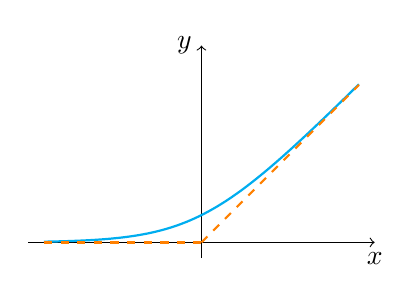
\begin{tikzpicture}
\draw[->] (-2.2,0) -- (2.2,0) node[below] {$x$};
\draw[->] (0,-0.2) -- (0,2.5) node[left] {$y$};
\draw[cyan,smooth,thick,domain=-2:2] plot(\x,{ln(1+e^(2*\x))/2});
\draw[orange,thick,dashed,domain=0:2] plot(\x,{\x});
\draw[orange,thick,dashed,domain=-2:0] plot(\x,{0});
\end{tikzpicture}
\end{minipage}
\end{frame}

\begin{frame}[label=softmax]
\frametitle{Softmax}
Derived from softmax regression, extension of logistic regression for multi-label classfication.
\begin{equation*}
y_{i}=\frac{e^{x_{i}}}{\sum_{k=1}^{n}e^{x_{k}}},\forall i\in[n]
\end{equation*}
Outputs of softmax layer are probabilities of each label.
\end{frame}

\begin{frame}
\frametitle{MNIST Database}
MNIST: Mixed National Institute of Standards and Technology
\begin{figure}[htbp]
\centerline{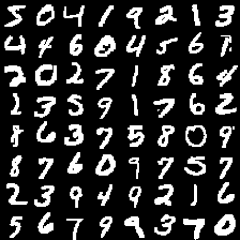
\includegraphics[width=.4\textwidth]{mnist.png}}
\caption[]{Handwritten Digits}
\end{figure}
10 distinguishing classes
\end{frame}

\begin{frame}[label=review]
\frametitle{LeNet Review}
\begin{figure}[htbp]
\centerline{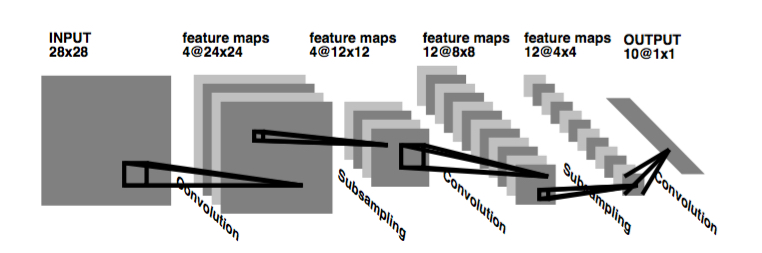
\includegraphics[width=\textwidth]{lenet.jpg}}
\caption[3]{LeNet for MNIST}
\end{figure}\par
\begin{itemize}
\item input: a picture (size $28\times 28$)
\item conv1: 4 kernels (size $5\times 5$)
\item pool1: max pooling (size $2\times 2$)
\item conv2: 3 kernels (size $5\times 5$)
\item pool2: max pooling (size $2\times 2$)
\item ip: full-connected ($192\to 10$)
\item softmax: 10 inputs, 10 prob outputs 
\end{itemize}
\end{frame}

\section{Caffe for CNN}
\begin{frame}
\frametitle{Caffe Tutorial}
For more information please refer to \href{http://furoc.net/2015/10/18/caffe\_learning/}{\color{blue}{this page}}.\par
Key words:\par
\begin{itemize}
\item \hyperlink{net}{Nets, Layers and Blobs}
\item \hyperlink{ward}{Forward / Backward}
\item \hyperlink{loss}{Loss}
\item \hyperlink{solver}{Solver}
\item \hyperlink{cata}{Layer Catalogue}
\item Interfaces
\item Data
\end{itemize}
\end{frame}

\begin{frame}[label=net]
\frametitle{Nets, Layers and Blobs}
\begin{minipage}[h]{\textwidth}
\begin{tikzpicture}
\node[anchor=south west,inner sep=0] at (0,0) {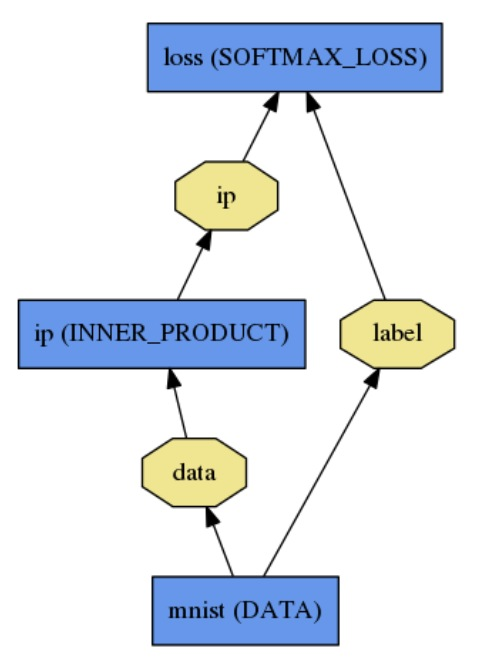
\includegraphics[width=.5\textwidth]{logreg.jpg}};
\draw[orange,thick] (2.5,3.5) ellipse (2.5 and 3.5);
\node[right,orange] at (5,3.5) {Net};
\draw[orange,->] (4.5,3) -- (6,1.5) node[right,orange] {Blob};
\draw[orange,->] (5,6.2) -- (7,6.2) node[right,orange] {Layer};
\node[left] at (10,0) {Example: Softmax Regression};
\end{tikzpicture}
\end{minipage}
\end{frame}

\begin{frame}[label=ward]
\frametitle{Forward / Backward}
\begin{minipage}[h]{\textwidth}
\begin{tikzpicture}
\node[anchor=south west,inner sep=0] at (3,0) {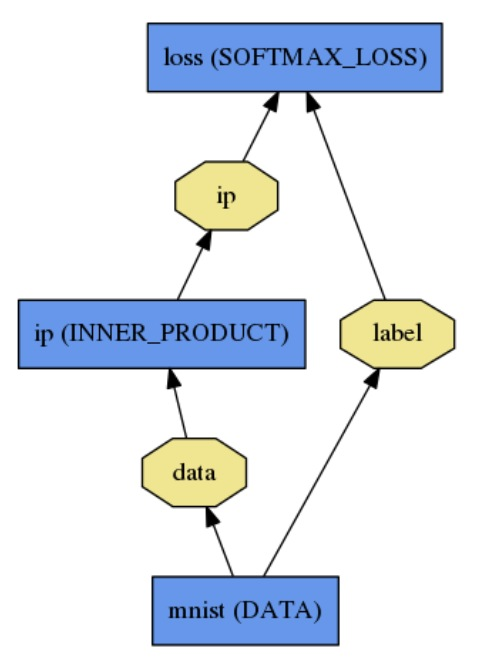
\includegraphics[width=.5\textwidth]{logreg.jpg}};
\draw[orange,thick,->] (3,7.2) -- (5,7.2);
\node[right] at (5,7.2) {$L(f(w^{T}x))$};
\draw[orange,thick,->] (2,4) -- (2,6.8);
\node[] at (2,3.5) {$w^{T}x$};
\node[above] at (2,6.8) {$f(w^{T}x)$};
\draw[orange,thick,->] (2,0.8) -- (2,3);
\node[below] at (2,0.8) {$x$};
\draw[orange,thick] (7.2,7.2) -- (9.5,7.2);
\draw[orange,thick,->] (9.5,7.2) -- (9.5,6.5);
\node[below] at (9.5,6.5) {$\frac{\partial L}{\partial f}$};
\draw[orange,thick,->] (9.5,5.5) -- (9.5,4);
\node[below] at (9.5,4) {$\frac{\partial L}{\partial w}$};
\end{tikzpicture}
\end{minipage}
\end{frame}

\begin{frame}[label=loss]
\frametitle{Loss}
Softmax:
\begin{equation*}
y_{i}(x)=\frac{e^{x_{i}}}{\sum_{k=1}^{n}e^{x_{k}}},\forall i\in[n]
\end{equation*}
Softmax loss function:\par
let label $j$ be groundtruth, therefore
\begin{equation*}
L=-ln(y_{j}(x))=-ln(\frac{e^{x_{j}}}{\sum_{k=1}^{n}e^{x_{k}}})=ln(\sum_{k=1}^{n}e^{x_{k}})-x_{j}
\end{equation*}
\begin{equation*}
\frac{\partial L}{\partial x_{i}}=y_{i}(x)-\delta_{ij}
\end{equation*}
where $\delta_{ij}=1$ iff $i=j$, and $\delta_{ij}=0$ otherwise.
\end{frame}


\begin{frame}[label=solver]
\frametitle{Solver}
SGD (Stochastic Gradient Descent)
\begin{eqnarray*}
w_{t+1}&=&w_{t}+\Delta w_{t}\\
\Delta w_{t+1}&=&\mu\Delta w_{t}-\alpha\frac{\partial L}{\partial w_{t}}
\end{eqnarray*}
$\alpha$: learning rate\par
$\mu$: momentum
\end{frame}

\begin{frame}
\frametitle{Solver}
Solver parameters (i.e.):
\begin{itemize}
\item basic learning rate: $\alpha=0.01$
\item learning rate policy: step (reduce learning rate according to step size)
\item step size: 100000
\item gamma: 0.1 (multipy learning rate with factor 0.1 after step size)
\item momentum: $\mu=0.9$
\item max iteration: 350000 (stop at iteration 350000)
\end{itemize}
\end{frame}

\begin{frame}[label=cata]
\frametitle{Layer Catalogue}
Please refer to \href{http://caffe.berkeleyvision.org/tutorial/layers.html}{\color{blue}{this page}}.\par
Vision layer:
\begin{itemize}
\item convolution
\item pooling
\end{itemize}
Loss layer:
\begin{itemize}
\item softmax loss
\item Euclidean loss
\item cross-entropy
\end{itemize}
Activation layer:
\begin{itemize}
\item sigmoid
\item ReLU
\item hyperbolic tangent
\end{itemize}
\end{frame}

\begin{frame}
\frametitle{Layer Catalogue}
Data layer:
\begin{itemize}
\item datebase
\item in-memory
\item HDF5 input
\item HDF5 output
\end{itemize}
Common layer:
\begin{itemize}
\item inner product
\item splitting
\item flatening
\item reshape
\item concatenation
\end{itemize}
\end{frame}

\section{Using Caffe - An Example}
\begin{frame}
\frametitle{Installation}
\textbf{Prerequisites}:\par
\hspace{30pt}protobuf, CUDA, OpenBLAS, Boost, OpenCV, lmdb, leveldb, cuDNN(optional), Python(optional), numpy(optional), MATLAB(optional)\par
\vspace{5pt}
\textbf{Install}:\par
\hspace{30pt}git clone git://github.com/BVLC/caffe /your/own/caffe/folder\par
\vspace{5pt}
\textbf{Go to Caffe root folder}\par
\hspace{30pt}cp Makefile.config.example Makefile.config\par
\hspace{30pt}make all\par
\hspace{30pt}make test\par
\hspace{30pt}make runtest\par
\vspace{5pt}
\textbf{Hardware}:\par
\hspace{30pt}K40, K20, Titan for ImageNet scale\par
\hspace{30pt}GTX series or GPU-equipped MacBook Pro for small datasets
\end{frame}

\begin{frame}
\frametitle{LeNet Example}
\hyperlink{review}{LeNet Structure}\par
\vspace{10pt}
\textbf{1. Protobuf Protocol}\par
\vspace{10pt}
\textbf{2. Run!}
\end{frame}

\begin{frame}
\frametitle{How to be Professional?}
1. Figure out theoretical keypoints (read papers)\par
2. Read Caffe source code\par
3. Be proficient at programming and debugging skills\par
4. Take advantage of search engine and community\par
5. Do it through this pipeline:
\begin{itemize}
\item Experiment design
\item Data preparation (build database with tools)
\item Model selection (including network and solver)
\item Training
\item Analysis and comparison
\end{itemize}
\end{frame}

\end{document}